\documentclass[12pt]{article}
\usepackage[utf8]{inputenc}

\title{Searching a Binary Tree}
\author{Benny Chen}
\date{October 21, 2022}

\usepackage{color}
\usepackage{amsthm}
\usepackage{amssymb} 
\usepackage{amsmath}
\usepackage{listings}
\usepackage{xcolor}
\usepackage{listings}
\usepackage{graphicx}
\usepackage[hidelinks]{hyperref}

\newtheorem{Definition}{Definition}
\begin{document}

\maketitle

\section{Introduction}
Binary trees are a kind of data structure used in computer science.
They are used to store data in a way that allows for fast searching.
They store data in a tree-like structure, where each node has at most two children that branch off of it.
The left child is always less than the parent, and the right child is always greater than the parent.
This allows for fast searching, as you can compare the value you are searching for to the value of the current node, and then search the left or right child depending on the result.
There are many algorithms and ways to search a binary tree like
a linear search, breadth-first search, and depth-first search.
In this paper, we will be looking at depth-first search, which is a recursive algorithm that searches the left child, then the right child, then the parent.
This algorithm is very efficient, as it only needs to search the tree once, and it will find the value if it exists.
In section 2, we will look at the algorithm for depth-first search and prove its correctness.
In section 3, we will look at the time and space complexity of depth-first search.
In section 4, we will look at how depth-first search can be used to solve a problem.

\begin{figure}[h!]
    \centering
    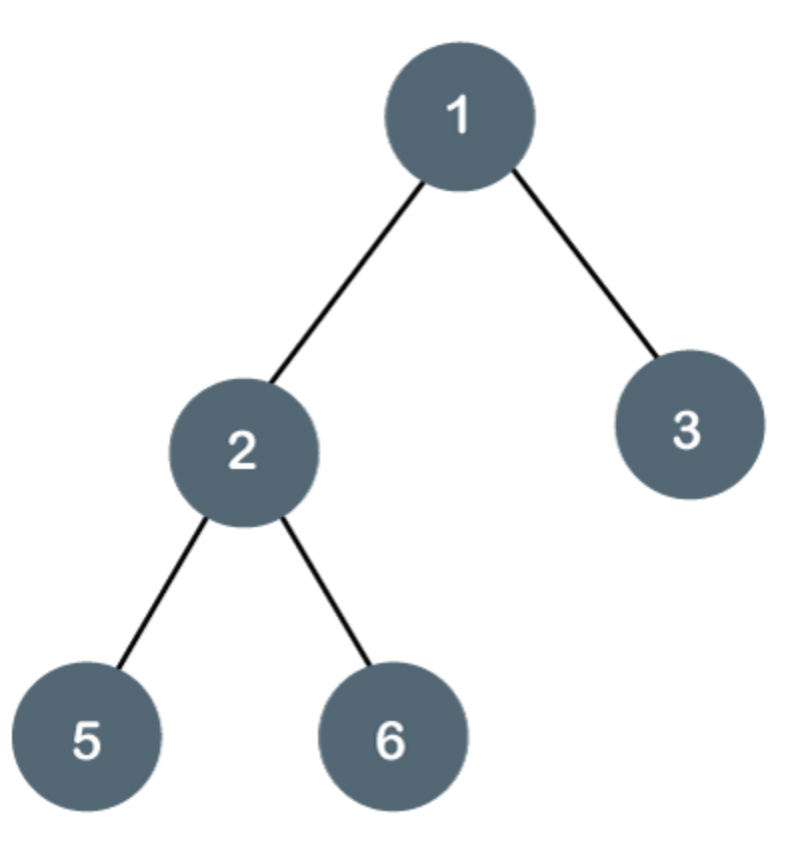
\includegraphics[scale=.196]{images/tree.png}
    \caption{Simple binary tree 1, 2, 3, 4, 5, 6} 
\end{figure}

\section{Preliminaries}
\begin{Definition}
    A binary tree is a data structure that stores data in a tree-like structure.
    Each node has at most two children, and the left child is always less than the parent, and the right child is always greater than the parent.
\end{Definition}
\begin{figure}[h!]
    \centering
    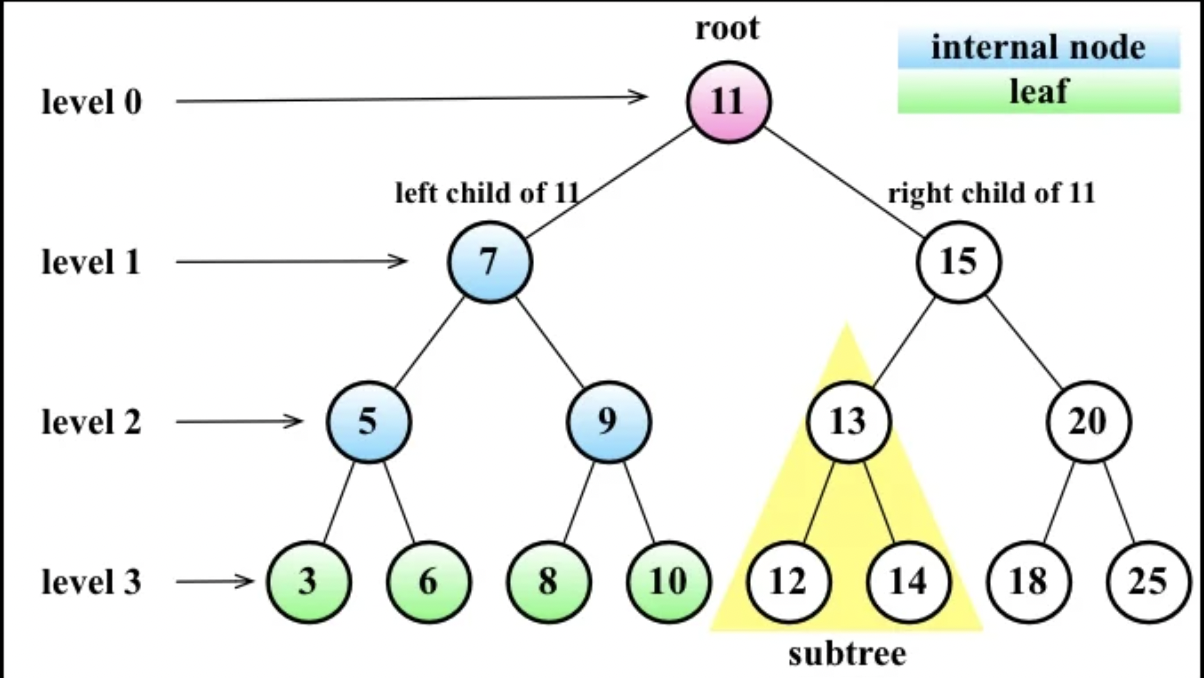
\includegraphics[scale=.6]{images/termen.png}
    \caption{Sample binary tree with showing subtree and values}
\end{figure}

\section{The Algorithm}

Depth-first search is a recursive algorithm that searches the left child, then the right child, then the parent.
As the name suggests, it searches the tree in a depth-first manner which means it checks the deepest nodes first.
The algorithm is as follows:
\begin{enumerate}
    \item If the current node is null, return false.
    \item If the current node's value is equal to the value we are searching for, return true.
    \item If the current node's value is greater than the value we are searching for, return the result of depth-first search on the left child.
    \item If the current node's value is less than the value we are searching for, return the result of depth-first search on the right child.
\end{enumerate}
\begin{figure}[h!]
    \centering
    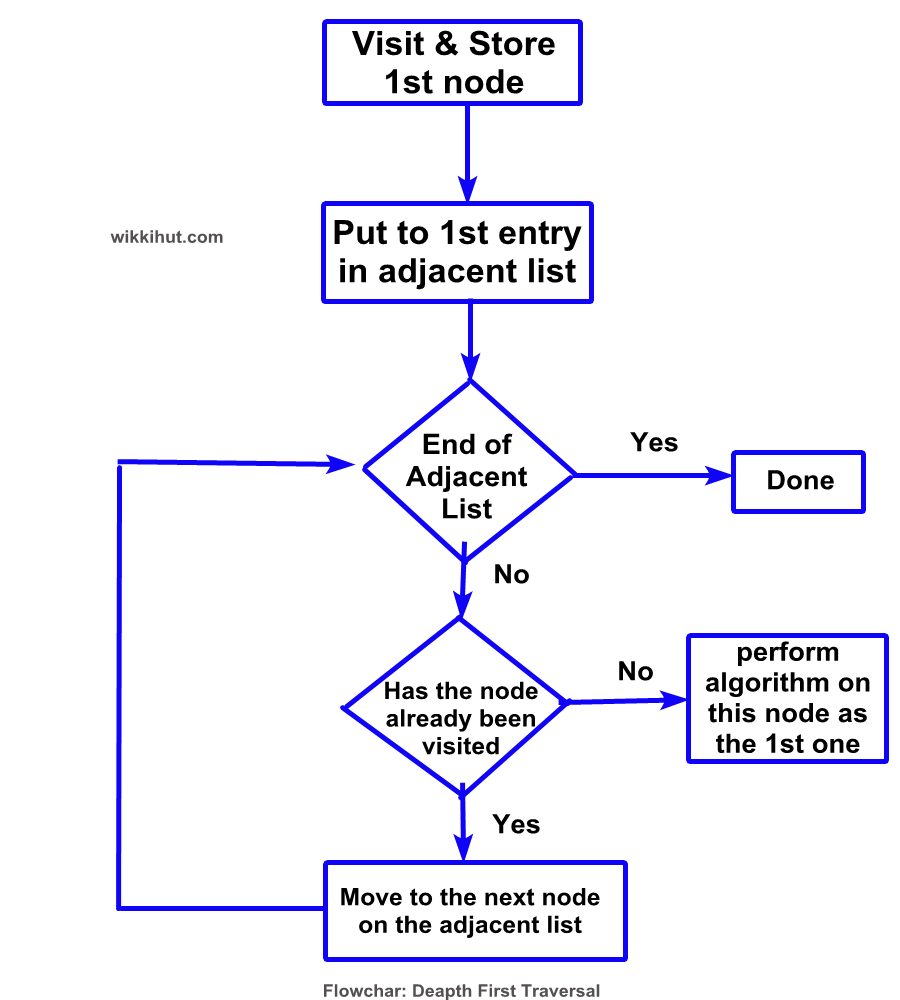
\includegraphics[scale=.4]{images/flowchart.png}
    \caption{Flowchart of depth-first search}
\end{figure}
A depth first search algorithm has a base case, which is when the current node is null or nothing.
This means that the value we are searching for is not in the tree, so we return false.
We can figure out the time complexity or the number of steps it takes to search the tree by looking at the number of nodes in the tree.
If we assume $V$ as the number of nodes in the tree or vertices and $E$ as the number of edges in the tree.
Along with $e$ as the number of edges to the current node and 1 as the node we are currently on.
We can derive a equation $T(V, E) = 1 + e_0 + T(V - e_0, E - e_0)$ to find the time complexity of depth-first search.
From this equation, if we keep expanding the equation with any arbitrary amount of nodes, we get 
$T(V, E) = 1 + 1 + ... + 1 + e_0 + e_1 + ... + e_V$. From this we can simplify the equation to $T(V, E) = V + E$.
This means that the time complexity of depth-first search is $O(V + E)$ or $O(n)$ where $n$ is the number of nodes in the tree.

\begin{figure}[h!]
    \centering
    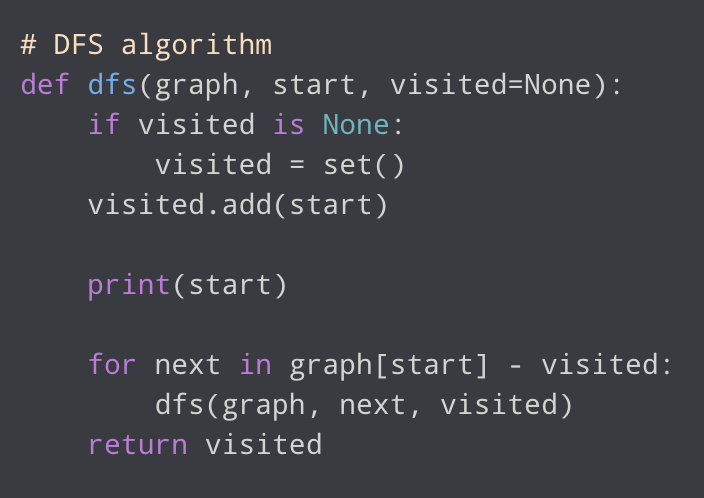
\includegraphics[scale=.75]{images/code.png}
    \caption{Sample code for depth-first search}
\end{figure}

\newpage
\section{Searching a Tree}
Depth-first search as stated before is a recursive algorithm that searches the left child, then the right child, then the parent.
This means that we search all the left side before checking the right side.
This can be used to solve a problem where we are given a binary tree and we need to find the sum of all the nodes in the tree.
This also can be used to find a specific node in the tree.
\begin{figure}[h!]
    \centering
    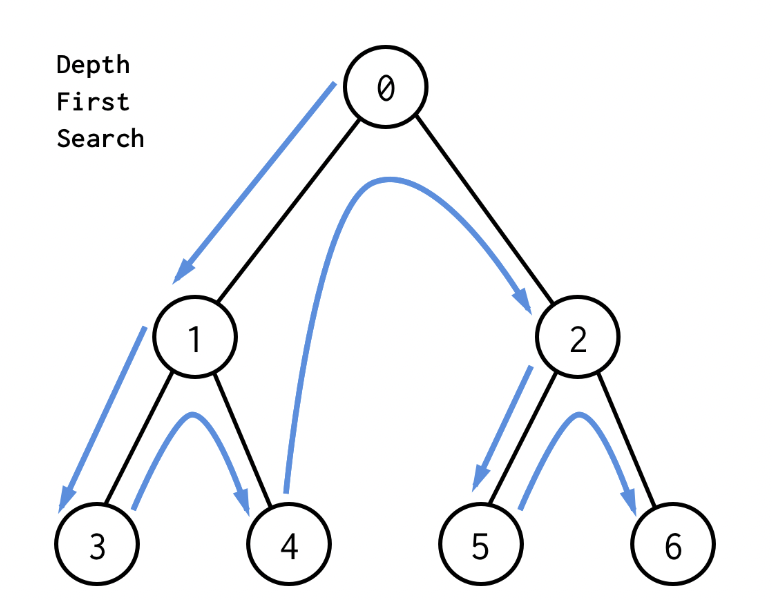
\includegraphics[scale=.5]{images/traversal.png}
    \caption{Depth-first search traversal}
\end{figure}
Depth first search can be used for many things, not just searching a tree.
For example, it can be used to find a path for a maze.
In this example, we will look at how depth-first search can be used to find a path for a maze.
\begin{figure}[h!]
    \centering
    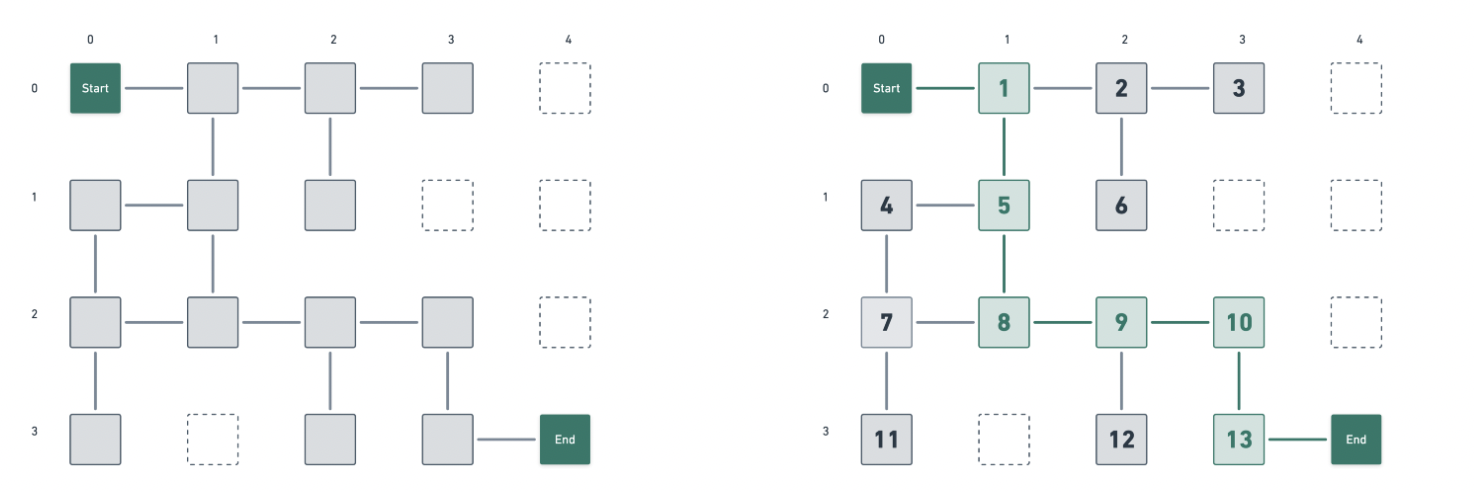
\includegraphics[scale=.5]{images/maze.png}
    \caption{Navigating a maze}
\end{figure}
In this maze, we are given a start and an end point.
We can basically check every possible path from the start point to the end point.
We can check a possible path then check if it is a dead end, if it is, we can backtrack and check another path.
If we find a path that leads to the end point, we can return that path.
This is a very simple example of how depth-first search can be used to solve a problem.
On a larger scale we can use this same exact problem to find a best path on a map or a graph.
This can now be used in the real world to find the best path to take to get to a destination.
There are many other algorithms that act similarly to depth-first search to both search a tree and to find a path.
For example, breadth-first search, which is a algorithm that insted of searching by side, searches by level.
Some may prefer breadth-first search over depth-first search for their use case but both are the same time complexity.

\begin{thebibliography}{9}
    \bibitem{website:https://wikkihut.com/depth-first-traversal/}
    https://wikkihut.com/depth-first-traversal/

    \bibitem{https://dev.to/danimal92/difference-between-depth-first-search-and-breadth-first-search-6om}
    https://dev.to/danimal92/difference-between-depth-first-search-and-breadth-first-search-6om

    \bibitem{https://www.programiz.com/dsa/graph-dfs}
    https://www.programiz.com/dsa/graph-dfs

    \bibitem{https://makeschool.org/mediabook/oa/tutorials/trees-and-mazes/generating-a-maze-with-dfs/}
    https://makeschool.org/mediabook/oa/tutorials/trees-and-mazes/generating-a-maze-with-dfs/

    \bibitem{https://subscription.packtpub.com/book/web-development/9781785285493/8/ch08lvl1sec55/tree-terminology}
    https://subscription.packtpub.com/book/web-development/9781785285493/8/ch08lvl1sec55/tree-terminology
    
\end{thebibliography}

\end{document}